\documentclass[tikz,border=10pt]{standalone}
% Only the calc library is needed (none used here, kept minimal)
\begin{document}
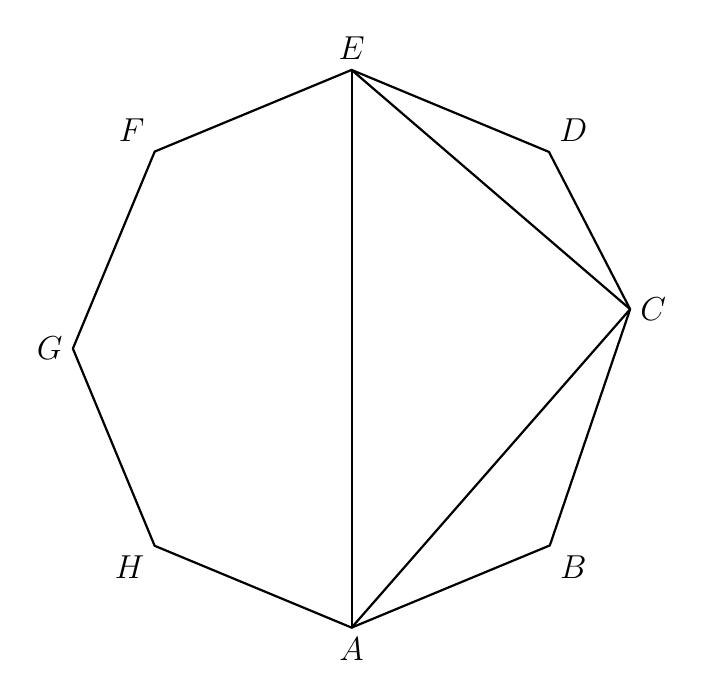
\begin{tikzpicture}[line join=round, line cap=round, line width=0.8pt,
  every node/.style={font=\fontsize{11.5}{13.8}\selectfont}]
  % Vertices of the regular octagon (pixel-derived, y up, scale 0.01 cm/px,
  % centred on the ink bbox centre (456.5, 452.5) px)
  \coordinate (A) at (-0.0024622793663398373,-3.5388245359133945);
  \coordinate (B) at (2.5150139135773006,-2.4950335575793554);
  \coordinate (C) at (3.5349999999999997,0.505);
  \coordinate (D) at (2.5039746987587854,2.5025320505006245);
  \coordinate (E) at (-0.0024635483718241148,3.543823268629186);
  \coordinate (F) at (-2.5028431770647637,2.507120833803686);
  \coordinate (G) at (-3.5423402127762404,0.005001270394034293);
  \coordinate (H) at (-2.5038793947569173,-2.4996193298347826);

  % Octagon sides (solid)
  \draw (A) -- (B) -- (C) -- (D) -- (E) -- (F) -- (G) -- (H) -- cycle;

  % Interior segments: vertical E-A and diagonals A-C, E-C
  \draw (E) -- (A);
  \draw (A) -- (C);
  \draw (E) -- (C);

  % Labels placed outside each vertex
  \node[below]       at (A) {$A$};
  \node[below right] at (B) {$B$};
  \node[right]       at (C) {$C$};
  \node[above right] at (D) {$D$};
  \node[above]       at (E) {$E$};
  \node[above left]  at (F) {$F$};
  \node[left]        at (G) {$G$};
  \node[below left]  at (H) {$H$};
\end{tikzpicture}
\end{document}